\documentclass[12pt]{article}  \usepackage[boxruled,lined]{algorithm2e} \usepackage{booktabs}
\usepackage{amsmath} \usepackage{amsthm} \usepackage{amsfonts} \usepackage{bbm} \usepackage{color,soul} \usepackage{framed} \usepackage[margin=0.5in]{geometry} \usepackage{hyperref} \usepackage{mathtools}
\usepackage[dvipsnames]{xcolor}
\usepackage{tikz}  
\usetikzlibrary{positioning}

\newtheorem{theorem}{Theorem}[section] \newtheorem{lemma}[theorem]{Lemma} \newtheorem{proposition}[theorem]{Proposition} \newtheorem{corollary}[theorem]{Corollary}  \DeclarePairedDelimiter{\ceil}{\lceil}{\rceil} \DeclarePairedDelimiter{\floor}{\lfloor}{\rfloor} \DeclareMathOperator*{\argmin}{arg\,min} \DeclareMathOperator*{\argmax}{arg\,max} \newcommand{\D}{\mathrm{d}} \SetKwInput{KwInput}{Input} \SetKwInput{KwOutput}{Output}  \begin{document}
\renewcommand{\d}[1]{\ensuremath{\operatorname{d}\!{#1}}}

\section{Logistic Regression}\vspace{.1pt} \hrule height 2pt \smallskip \renewcommand{\arraystretch}{1}% Tighter \begin{description} \item[Intro] 
This model assumes that the log odds-ratio can be fit by a linear model. We start with the probability mass function for a \href{https://en.wikipedia.org/wiki/Bernoulli_distribution}{Bernoulli trial}: $f(y;p) = p^y \times (1-p)^{(1-y)}$ for $y \in \{0, 1\}$. We are interested in estimating what $p$ is, and so it's natural to conceive of a maximum likelihood estimator; since $\log$ monotone we can apply this transformation without changing the maximizer. The log-likelihood is given by $y \log p + (1-y) \log (1-p)$ using \href{https://en.wikipedia.org/wiki/Logarithm#Logarithmic_identities}{properties of logarithms}. In optimization, we generally work to minimize objective functions, and so it's then natural to set our (objective) \emph{loss function}
to be $- \left[y \log p + (1-y) \log (1-p)\right]$. In summary, we 
have, for $\sigma(x) = \frac{1}{1 + \exp(-x)}$:
\begin{align}
  z &= w^Tx + b \\
  \hat y &= a = \sigma(z) \\
  \mathcal{L}(a, y) &= - \left[y \log (a) + (1-y) \log (1-a)\right] \end{align}

We can draw a \emph{computation graph} to describe the forward pass as follows:
\begin{center}
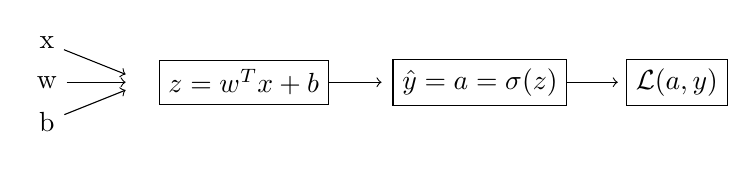
\begin{tikzpicture}
  \node (x) at (0, 1) {x};
  \node (w) at (0,.5) {w};
  \node (b) at (0, 0) {b};
  \draw[->] (x) to (1, .6);
  \draw[->] (w) to (1, .5);
  \draw[->] (b) to (1, .4);
  \node[draw=black,rectangle] (z) at (2.5, .5) {$z = w^Tx + b$};
  \draw[->] (z) to (4.25, .5);
  \node[draw=black,rectangle] (yhat) at (5.5, .5) {$\hat y = a = \sigma(z)$};
  \draw[->] (yhat) to (7.25, .5);
  \node[draw=black,rectangle] (loss) at (8, .5) {$\mathcal L (a,y)$};
\end{tikzpicture}
\end{center} We seek to learn $w, b$ to minimize the loss function. \emph{Back propogation} proceeds as follows:

{
\small{
\begin{align*}
\texttt{da} &= \frac{\partial \mathcal L}{\partial a} = - \left(\frac{y}{a} - \frac{1-y}{1-a}\right) = \frac{-y}{a} + \frac{1-y}{1-a}. \\
  \texttt{dz} &= \frac{\partial \mathcal L}{\partial z} = \frac{\partial \mathcal L}{\partial a}\frac{\partial a}{\partial z} = \left(\frac{-y}{a} + \frac{1-y}{1-a}\right) \times a(1-a) = \frac{-y}{a} \cdot a(1-a) + \frac{1-y}{1-a} \cdot (1-a) a = -y(1-a)+ (1-y)a \\ &= ay - y + a - ay = a - y.  \\
\texttt{dw} &= \frac{\partial \mathcal L}{\partial w} \overset{?}{=} \frac{\partial \mathcal L}{\partial z} \frac{\partial z}{\partial w} = (a-y) x^T. \\
\texttt{db} &= \frac{\partial \mathcal L}{\partial b} = \frac{\partial \mathcal L}{\partial z} \underbrace{\frac{\partial z}{\partial b}}_{=1}. \end{align*}
}
}
Our update rule then becomes: $w := w - \alpha \texttt{dw}$, and $b := b - \alpha \texttt{db}$. Our (average) \emph{cost} function is defined as $J(w,b) = \frac{1}{m} \sum_{i=1}^m \mathcal L(a^{(i)}, y^{(i)})$. Since $\frac{\partial}{\partial \cdot}$ is a linear operator, obtaining gradients is quite straightforward since we are left with a series of derivatives of loss functions, which we calculated above.
\begin{align*}    \frac{\partial J}{\partial w} = \frac{1}{m} \sum \frac{\partial \mathcal L}{\partial w}, \hspace{15pt} \textrm{and} \hspace{15pt} \frac{\partial J}{\partial b} = \frac{1}{m} \sum \frac{\partial \mathcal L}{\partial b} \end{align*}
Our optimization routine then can be written as in algorithm \ref{alg: logisticreg}

{\small
\begin{algorithm}[H]
  \label{alg: logisticreg}
  \caption{Logistic Regression - Optimization}   \For{\texttt{i in range(m)}} {
    $z^{(i)} = w^Tx^{(i)} + b$ \\
    $a^{(i)} = \sigma(z^{(i)})$ \\
    $J += - \left[ y^{(i)} \log a^{(i)} + (1-y^{(i)}) \log (1 - a^{(i)}) \right]$ \\
    $\partial d z^{(i)} = a^{(i)} - y^{(i)}$ \\
    $\partial d w += \partial d z^{(i)} {x^{(i)}}^T$ \\
    $\partial d b += \partial d z^{(i)}$
}
$J /= m$ \\
$\partial w /= m$ \\
$\partial b /= m$ \end{algorithm}
}
The above concludes one round of \href{https://en.wikipedia.org/wiki/Gradient_descent}{Gradient Descent}. We repeat this procedure many times until training loss (and ideally test loss ) is sufficiently minimized. We remark that it's possible to remove both \texttt{for} loops (over the training data, and over the parameters in $w$) by using vectorized operations in \texttt{numpy}. We execute this in code \href{https://github.com/asantucci/NN/blob/master/logistic_regression.py#L46}{here}.

\section{Neural Networks with 2-layers}
\vspace{-10pt}
We previously saw a simple computation graph. 
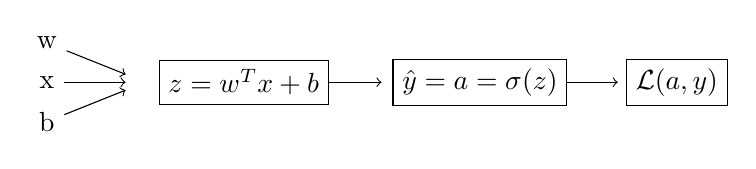
\begin{tikzpicture}   \node (w) at (0, 1) {w};
  \node (x) at (0, .5) {x};
  \node (b) at (0,0) {b};
  \draw[->] (x) to (1, .5);
  \draw[->] (w) to (1, .6);
  \draw[->] (b) to (1, .4);
  \node[draw=black,rectangle] (z) at (2.5, .5) {$z = w^Tx + b$};
  \draw[->] (z) to (4.25, .5);
  \node[draw=black,rectangle] (yhat) at (5.5, .5) {$\hat y = a = \sigma(z)$};
  \draw[->] (yhat) to (7.25, .5);
  \node[draw=black,rectangle] (loss) at (8, .5) {$\mathcal L (a,y)$};
\end{tikzpicture}
\subsection{Understanding Small Neural Networks}
A Neural Network can be constructed by stacking together sigmoids, depicted as follows:
\begin{figure}[h]
\centering
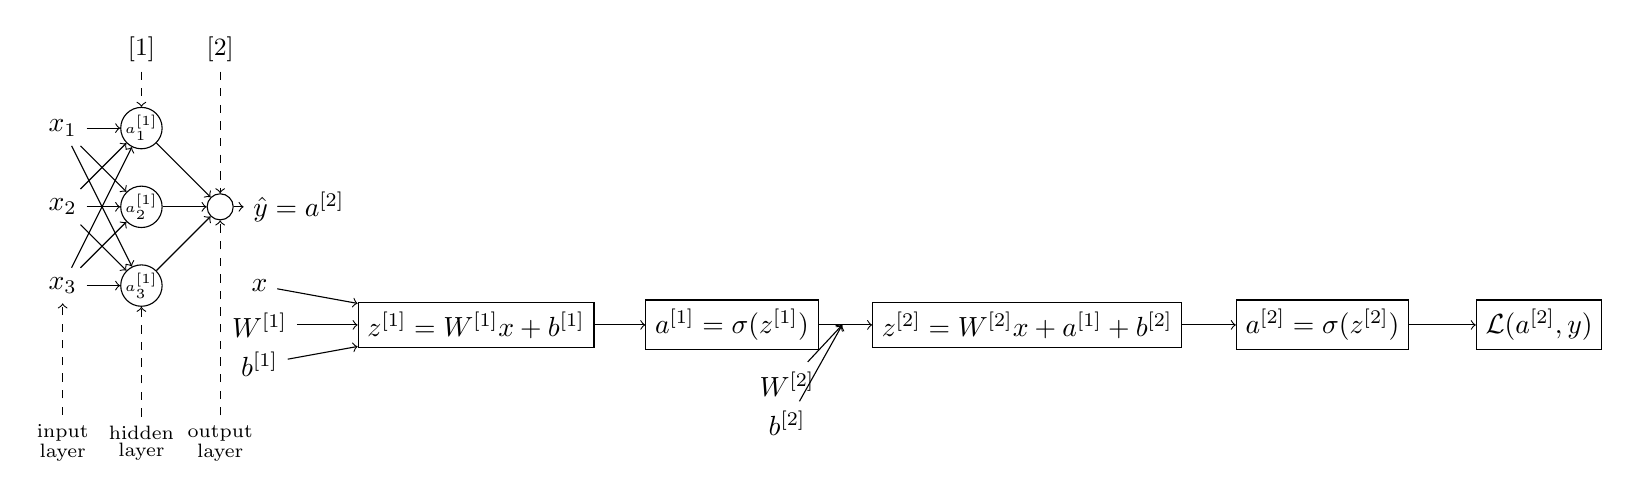
\begin{tikzpicture}
  \node (x1) at (0, 1) {$x_1$};
  \node (x2) at (0, 0) {$x_2$};
  \node (x3) at (0,-1) {$x_3$};
  \node (inputlayer) at (0, -3) {$\substack{\textrm{input}\\ \textrm{layer}}$};
  \draw[->,dashed] (inputlayer) to (x3);
  \node (lbl) at (1,2) {\small{$[1]$}}; 
  \node[draw=black,circle,inner sep = 0pt] (n1) at (1, 1) {\tiny $a_1^{[1]}$};
  \draw[->,dashed] (lbl) to (n1);
  \node[draw=black,circle,inner sep = 0pt] (n2) at (1, 0) {\tiny $a_2^{[1]}$};
  \node[draw=black,circle,inner sep = 0pt] (n3) at (1,-1) {\tiny $a_3^{[1]}$};
  \node (hiddenlayer) at (1, -3) {$\substack{\textrm{hidden}\\ \textrm{layer}}$};
  \draw[->,dashed] (hiddenlayer) to (n3);
  \draw[->] (x1) to (n1);
  \draw[->] (x1) to (n2);
  \draw[->] (x1) to (n3);   \draw[->] (x2) to (n1);
  \draw[->] (x2) to (n2);
  \draw[->] (x2) to (n3);   
  \draw[->] (x3) to (n1);
  \draw[->] (x3) to (n2);
  \draw[->] (x3) to (n3); 
  \node[draw=black,circle] (m1) at (2,0) {};
  \node (lbl2) at (2,2) {\small{$[2]$}}; 
  \draw[->,dashed] (lbl2) to (m1);
  \node (yhat) at (3,0) {$\hat y = a^{[2]}$};
  \node (outputlayer) at (2, -3) {$\substack{\textrm{output}  \\ \textrm{layer}}$};
  \draw[->,dashed] (outputlayer) to (m1);
  \draw[->] (n1) to (m1);
  \draw[->] (n2) to (m1);
  \draw[->] (n3) to (m1);
  \draw[->] (m1) to (yhat);
  \node (x) at (2.5, -1) {$x$};
  \node (w1) at (2.5, -1.5) {$W^{[1]}$};
  \node (b1) at (2.5, -2) {$b^{[1]}$};
  \node[draw=black,rectangle] (z1) at (5.25, -1.5) {$z^{[1]} = W^{[1]}x + b^{[1]}$};
  \draw[->] (x) to (z1);
  \draw[->] (w1) to (z1);
  \draw[->] (b1) to (z1);
  \node[draw=black,rectangle] (a1) at (8.5, -1.5) {$a^{[1]} = \sigma (z^{[1]})$};
  \draw[->] (z1) to (a1);
  \node[draw=black,rectangle] (z2) at (12.25, -1.5) {$z^{[2]} = W^{[2]}x + a^{[1]} + b^{[2]}$};
  \draw[->] (a1) to (z2);
  \node (w2) at (9.2, -2.25) {$W^{[2]}$};
  \node (b2) at (9.2, -2.75) {$b^{[2]}$};
  \draw[->] (w2) to (9.9, -1.5);
  \draw[->] (b2) to (9.9, -1.5);
  \node[draw=black,rectangle] (a2) at (16, -1.5) {$a^{[2]} = \sigma(z^{[2]})$};
  \draw[->] (z2) to (a2);
  \node[draw=black,rectangle] (l) at (18.75, -1.5) {$\mathcal L(a^{[2]},y)$};
  \draw[->] (a2) to (l);
\end{tikzpicture}
\caption{A 2-layer Neural Network (you could say we don't count the input layer, or you could say we do but we index starting from zero).}
\end{figure}
\newline
\vspace{-40pt}
\paragraph{Terminology and Notation}
Each \emph{neuron} in the graph consists of both a linear transformation and a non-linear activation function, i.e. the first stack of nodes will produce a $z$ and an $a$. We use the super-script square brackets $[\hspace{2pt} ]$ to denote a stack of nodes, i.e. a layer, not to be confused with super-script parentheses which index training examples. I.e. $a^{[\ell]}_i$ denotes the output of an activation function in layer $\ell$ for the $i$th neuron.
The key difference between our Logistic Regression and 
this (or any) Neural Network is that we simply repeat linear transformations followed by non-linear activation functions \emph{multiple times}.
The reason why we call the intermediary layer a ``hidden'' layer is because we do not observe what these values are to be in the training set. By convention, we define  $a^{[0]} = X$. We can further refer to the hidden layer by ${a^{[1]}} = \begin{bmatrix}   a_1^{[1]} & a_2^{[1]} & a_3^{[1]}  \end{bmatrix}^T$. Notice that the hidden layer and output layer have parameters $W^{[\cdot]}$ and $b^{[\cdot]}$ associated with them. 

\paragraph{Visualizing a Neuron}
Let's take a look at neural network representation in a bit more detail. We can think about each neuron as being divided into two parts: one which performs a linear transformation and another which performs an activation function. The mental model is:
\begin{figure}[h]
  \centering   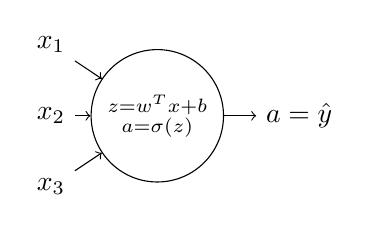
\begin{tikzpicture}[scale=0.9]     \node (x1) at (0, 1) {$x_1$};
    \node (x2) at (0, 0) {$x_2$};
    \node (x3) at (0,-1) {$x_3$};
    \node[draw,circle] (neuron) at (1.5,0) {$\substack{z = w^Tx + b \\ a = \sigma(z)}$};
    \draw[->] (x1) to (neuron);
    \draw[->] (x2) to (neuron);
    \draw[->] (x3) to (neuron);
    \node (output) at (3.5,0) {$a = \hat y$};
    \draw[->] (neuron) to (output);
  \end{tikzpicture} \end{figure}
\newline
In general, we'll have something as follows for the first neuron in the hidden layer, and to be crystal clear we draw out the second neuron as well.
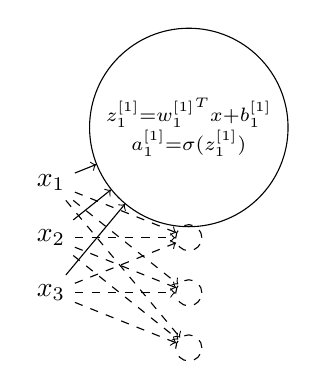
\begin{tikzpicture}[scale=0.7]     \node (x1) at (0, 1) {$x_1$};
    \node (x2) at (0, 0) {$x_2$};
    \node (x3) at (0,-1) {$x_3$};
    \node[draw,circle] (neuron) at (2.5,2) {$\substack{z_1^{[1]} = {w_1^{[1]}}^Tx + b_1^{[1]} \\ a_1^{[1]} = \sigma(z_1^{[1]})}$};
    \draw[->] (x1) to (neuron);
    \draw[->] (x2) to (neuron);
    \draw[->] (x3) to (neuron);
    \node[draw,circle,dashed] (n2) at (2.5,0 ) {};     \node[draw,circle,dashed] (n3) at (2.5,-1) {}; 
    \node[draw,circle,dashed] (n4) at (2.5,-2) {}; 
    \draw[->,dashed] (x1) to (n2);
    \draw[->,dashed] (x2) to (n2);
    \draw[->,dashed] (x3) to (n2);
    \draw[->,dashed] (x1) to (n3);
    \draw[->,dashed] (x2) to (n3);
    \draw[->,dashed] (x3) to (n3);
    \draw[->,dashed] (x1) to (n4);
    \draw[->,dashed] (x2) to (n4);
    \draw[->,dashed] (x3) to (n4);
\end{tikzpicture}
\hspace{20pt} 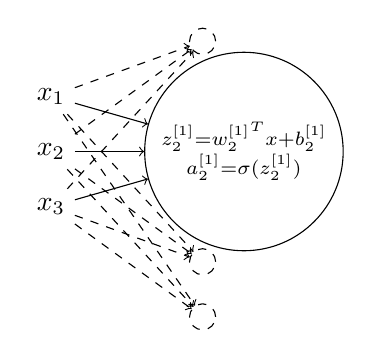
\begin{tikzpicture}[scale=0.7]     
    \node (x1) at (0, 1) {$x_1$};
    \node (x2) at (0, 0) {$x_2$};
    \node (x3) at (0,-1) {$x_3$};
    \node[draw,circle,dashed] (neuron) at (2.75,2) {};
    \draw[->,dashed] (x1) to (neuron);
    \draw[->,dashed] (x2) to (neuron);
    \draw[->,dashed] (x3) to (neuron);
    \node[draw,circle] (n2) at (3.5,0 ) {$\substack{z_2^{[1]} = {w_2^{[1]}}^Tx + b_2^{[1]} \\ a_2^{[1]} = \sigma(z_2^{[1]})}$};     
    \node[draw,circle,dashed] (n3) at (2.75,-2) {}; 
    \node[draw,circle,dashed] (n4) at (2.75,-3) {}; 
    \draw[->] (x1) to (n2);
    \draw[->] (x2) to (n2);
    \draw[->] (x3) to (n2);
    \draw[->,dashed] (x1) to (n3);
    \draw[->,dashed] (x2) to (n3);
    \draw[->,dashed] (x3) to (n3);
    \draw[->,dashed] (x1) to (n4);
    \draw[->,dashed] (x2) to (n4);
    \draw[->,dashed] (x3) to (n4);
\end{tikzpicture} 
To avoid having to calculate $z_i^{[\ell]}$ using a \texttt{for}
loop, we can instead use a matrix multiply.
$$
W^{[1]}x + b^{[1]} = 
\underbrace{\begin{bmatrix}    & {w_1^{[1]}}^T & \\
   & {w_2^{[1]}}^T & \\    & {w_3^{[1]}}^T & \\    
   & {w_4^{[1]}}^T & \\ 
\end{bmatrix}}_{\in \mathbb R^{4, 3}} \begin{bmatrix} x_1 \\ x_2 \\ x_3  \end{bmatrix} + \begin{bmatrix}   b_1^{[1]} \\ b_2^{[1]} \\ b_3^{[1]} \\ b_4^{[1]} \end{bmatrix} = \begin{bmatrix}   z_1^{[1]} \\
  z_2^{[1]} \\
  z_3^{[1]} \\
  z_4^{[1]} \\ \end{bmatrix} = z^{[1]}
$$

We can then write ${a^{[1]}}^T = \begin{bmatrix}   a_1^{[1]} & a_2^{[1]} & a_3^{[1]} & a_4^{[1]} \end{bmatrix} = \sigma (z^{[1]})$ where the $\sigma(\cdot)$ is applied element-wise.

To summarize, given an input $x$, we set $a^{[0]} = x$ and we compute forward steps: $z^{[\ell]} = W^{[\ell]}a^{[\ell-1]} + b^{[\ell]}$
for each layer in the network.

\paragraph{Vectorization} Suppose we have a single hidden-layer neural network. As per above, the forward propagation involves computing: 
$  z^{[1]} = W^{[1]}a^{[0]} + b^{[1]}; \hspace{10pt} a^{[1]} = \sigma(z^{[1]}); \hspace{10pt} 
   z^{[2]} = W^{[2]}a^{[1]} + b^{[2]}; \hspace{10pt} 
   a^{[2]} = \sigma(z^{[2]}).
$
We need to replicate this procedure for each of our $m$ training samples. I.e. we need to feed each training example through the network to get an output. Let our final output be denoted by $a^{[\ell](j)}$ denote the output for the activation function for the $j$th training example at the $\ell$th layer in our network. So in our case above, $a^{[2](j)}$ is the output for the $j$th training example.
To avoid a \texttt{for} loop over each of our $m$ training examples:
{\tiny
\begin{algorithm}[h]
  \caption{Naive Forward Propagation on a 2-layer Neural Network}   \For{i = 1 to m}{
    $z^{[1](i)} = W^{[1]}x^{(i)} + b^{[1]}$ \\
    $a^{[1](i)} = \sigma(z^{[1]}(i))$ \\
    $z^{[2](i)} = W^{[2]}a^{[1](i)} + b^{[2]}$ \\
    $a^{[2](i)} = \sigma(z^{[2]}(i))$
  } \end{algorithm}
}
\newline
\vspace{-.5ex}Recall we arranged our input matrix such that each column is an observation, i.e. $X = \begin{bmatrix}    | & | & & | \\    x^{(1)} & x^{(2)} & \ldots & x^{(m)} \\   | & | & & |  \end{bmatrix} \in \mathbb R^{n_x, m}$. Then,
$  
  Z^{[1]} = W^{[1]} X + b^{[1]}; \hspace{10pt}
  A^{[1]} = \sigma(Z^{[1]}); \hspace{10pt}
  Z^{[2]} = W^{[2]} A^{[1]} + b^{[2]}; \hspace{10pt}
  A^{[2]} = \sigma(Z^{[2]})
$ To be explicit, $Z^{[1]}$ is also arranged with observations in columns, i.e. $Z^{[1]} = \begin{bmatrix}   | & | & & | \\ z^{[1](1)} & z^{[1](2)} & \ldots & z^{[1](m)} \\ | & | & & | \end{bmatrix}$ and $A^{[1]} = \begin{bmatrix}    | & | & & | \\    a^{[1](1)} & a^{[1](2)} & \ldots & a^{[1](m)}  \\  | & | & & | \end{bmatrix}$.\footnote{As one scans matrix $A^{[\ell]}$ from left to right, we scan through observations or training examples, and as we scan from top to bottom we scan through the activations of different hidden units.}

\subsection{Activation Functions}
\paragraph{Hyperbolic Tangent}
Another activation function to consider is $\tanh (z) = \frac{e^z - e^{-z}}{e^z + e^{-z}}$. It's a shifted and rescaled version of the sigmoid function, which ranges from $[-1, 1]$ and cross the $x$-axis at zero; it is intuitively thought to perform better than a sigmoid activation function since it has the effect of ``centering'' the data in the intermediate layers of the network around zero. The one exception is the output layer: if we are predicting binary classification it makes sense to use sigmoid since our target values are in $\{0, 1\}$ we therefore want $\hat y$ to be in $(0,1)$.

\begin{figure}[h]
  \centering   \begin{tikzpicture}   \draw[->] (-3,0) -- (3,0) node[right] {$x$};   \draw[->] (0,-1) -- (0,1) node[above] {$y$};
  \draw[domain=-3:3,smooth,variable=\x,blue] plot ({\x},{(exp(\x) - exp(-\x))/(exp(\x) + exp(-\x))}); 
\end{tikzpicture}   \end{figure}
Both sigmoid and $\tanh$ suffer from the problem of saturating gradients. I.e. if the input value is either very small or very large, the derivative of the function becomes very small. This has the effect of slowing down gradient descent.

\paragraph{Rectified Linear Unit}
This leads us to the rectified linear unit: $a = g(z) = \max\{0, z\}$. The derivative at zero is not well defined, however, it is unlikely that we will ever encounter a true zero in our computations and so we can ignore this case without much worry. One disadvantage of the ReLU is that its derivative is identically zero when the input is negative, but this ends up not harming us in practice: enough neurons will likely have positive inputs such that gradients can still be learned. There is also the leaky ReLU: $a = g(z) = \max\{0.01 \times z, z\}$.

\begin{figure}[h]
  \centering   
  \begin{tikzpicture}   
    \draw[->] (-1,0) -- (1,0) node[right] {$x$};   
    \draw[->] (0,-1) -- (0,1) node[above] {$y$};
    \draw[domain=-1:1,smooth,variable=\x,blue] plot ({\x},{max(0,\x)}); 
  \end{tikzpicture}   
\end{figure}

\paragraph{Linear Activation Function (Identity Function)} It's worthwhile to realize that if we only used linear activation functions $g(z) = z$, then our neural network would in fact be a linear model. This is easy to see, since if $a^{[1]} = z^{[1]} = W^{[1]} x + b^{[1]}$ and $z^{[2]} = W^{[2]} a^{[1]} + b^{[2]}$ then plugging in for $a^{[1]}$, $z^{[2]} = W^{[2]} (W^{[1]} x + b^{[1]}) + b^{[2]} = \underbrace{W^{[2]}W^{[1]}}_{=W'}x + \underbrace{W^{[2]}b^{[1]} + b^{[2]}}_{b'}$ which is linear with respect to the input $x$. The one time we may use a linear activation function is if, for example, we were predicting housing prices, in which case we may want our output to range arbitrarily high. Even then, a better choice would be ReLU since housing prices are non-negative.

\subsubsection{Derivatives of Activation Functions} 
\paragraph{Hyperbolic Tangent}
Recall that 
\begin{align*}   \sinh(x) = \frac{e^x - e^{-x}}{2}, \hspace{10pt} 
  \cosh(x) = \frac{e^x + e^{-x}}{2}, \hspace{10pt} \textrm{ and } \hspace{5pt}
  \tanh(x) = \frac{\sinh(x)}{\cosh(x)}. \end{align*}
It's easy to see using linearity of $\frac{\d \,}{\d x}$ and the chain rule that $\frac{\d \,}{\d x}  \sinh(x) = \frac{e^x}{2} + \frac{e^{-x}}{2} = \cosh(x)$ and similarly that $\frac{\d \,}{\d x}\cosh(x) = \sinh(x)$. Then, apply either quotient rule \emph{or} both the product rule and chain rule:
\begin{align}   \frac{\d \,}{\d x} \tanh(x) = \frac{\d \,}{\d x} \sinh(x) \cosh(x)^{-1} = \cosh(x) \cosh(x)^{-1} - \sinh(x)\cosh(x)^{-2}\sinh(x) = 1 - \tanh(x)^2. \end{align}
\paragraph{Rectified Linear Unit} has derivative equal to
\begin{align}   \frac{\d \,}{\d x} \max\{0,x\}=       \begin{cases}        0 &\quad\text{if } x < 0\\        1 &\quad\text{if } x > 0 \\
       \textrm{undefined} &\quad\text{if } x = 0      \end{cases} \end{align}
Technically the derivative is undefined when $x = 0$, however, in practice a floating point variable never takes on the value zero exactly. We can therefore ignore this case by choosing to ``define'' the gradient to be either zero or one (which we choose again doesn't matter in practice). Either way, note that ReLU is convex and so we realize a \href{https://en.wikipedia.org/wiki/Subderivative}{sub-derivative}.

\paragraph{Leaky ReLU} is defined as $\max \{0.01 x, x \}$ and its derivative is therefore given by
\begin{align}   
  \frac{\d \,}{\d x} \max\{0.01x,x\}=       
  \begin{cases}        
    0.01 &\quad\text{if } x < 0\\        
    1    &\quad\text{if } x > 0 \\
    \textrm{undefined} &\quad\text{if } x = 0      
  \end{cases} 
\end{align}
Again the fact that the derivative doesn't exist at $x=0$ doesn't matter in practice since we're dealing with floating point values that are never identically zero.

\subsection{Back-Propagation for Neural Networks}
\paragraph{Review: Logistic Regression Computation Graph}
Recall our logistic regression computation graph. After computing our forward pass, we needed to compute a backward pass by calculating gradients at each step, depicted in \color{orange}{orange} \color{black} below.
\begin{figure}[h]
\centering 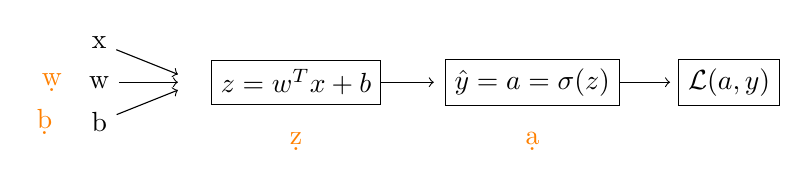
\begin{tikzpicture}
  \node (x) at (0, 1) {x};
  \node (w) at (0, .5) {w};
  \node (b) at (0,0) {b};
  \node [left = .1cm of w] {\color{orange}$\d w$}; 
  \node [left = .25cm of b] {\color{orange}$\d b$}; 
  \draw[->] (x) to (1, .6);
  \draw[->] (w) to (1, .5);
  \draw[->] (b) to (1, .4);
  \node[draw=black,rectangle] (z) at (2.5, .5) {$z = w^Tx + b$};
  \node at (2.5,-0.25) {\color{orange}$\d z$};
  \draw[->] (z) to (4.25, .5);
  \node[draw=black,rectangle] (yhat) at (5.5, .5) {$\hat y = a = \sigma(z)$};
  \node at (5.5,-0.25) {\color{orange}$\d a$};
  \draw[->] (yhat) to (7.25, .5);
  \node[draw=black,rectangle] (loss) at (8, .5) {$\mathcal L (a,y)$};
\end{tikzpicture}   \end{figure}
\newline
Note that $\d z = \d a \cdot g'(z)$ where $g(z) = \sigma(z)$, i.e. we use the fact that $\frac{\d L(a,y)}{\d z} = \frac{\d L(a,y)}{\d a} \frac{\d a}{\d z}$.

\paragraph{Two Layer Neural Network Back Propagation}
Let us now reconsider our two layer neural network and 
its computation graph. We highlight terms we must compute in \color{orange}{orange}\color{black}.
\begin{figure}[h]
\hspace{-20pt}
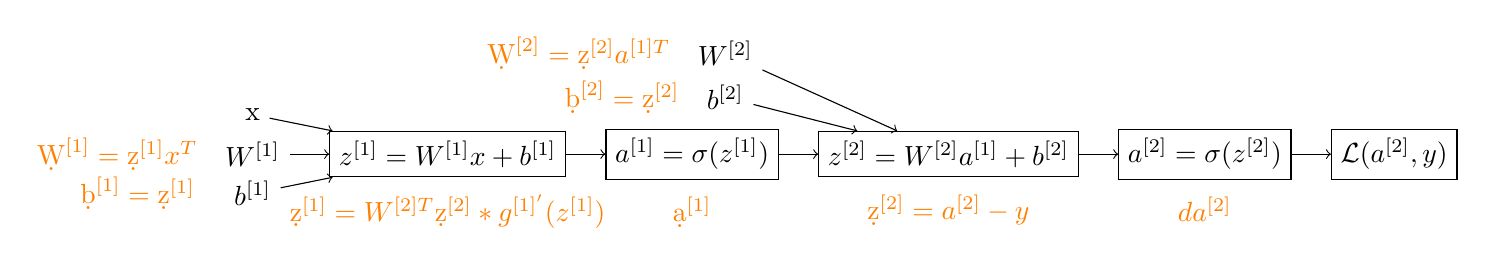
\begin{tikzpicture}
  \node (x)  at (-3, 1)  {x};
  \node (w1) at (-3, .5) {$W^{[1]}$};
  \node (b1) at (-3,0)   {$b^{[1]}$};
  \node [left = .1cm of w1] {\color{orange}$\d W^{[1]}= \d z^{[1]} x^T$}; 
  \node [left = .25cm of b1] {\color{orange}$\d b^{[1]}= \d z^{[1]}$}; 
  \node[draw=black,rectangle, right = .5cm of w1] (z1)  {$z^{[1]} = W^{[1]}x + b^{[1]}$};
  \draw[->] (x) to (z1);
  \draw[->] (w1) to (z1);
  \draw[->] (b1) to (z1);
  \node [below = .1cm of z1] {\color{orange}$\d z^{[1]}=W^{[2]T} \d z^{[2]} * g^{[1]'}(z^{[1]})$};
  \node[draw=black,rectangle, right = .5cm of z1] (a1) {$a^{[1]} = \sigma(z^{[1]})$};
  \draw[->] (z1) to (a1);
  \node [below = .1cm of a1] {\color{orange}$\d a^{[1]}$};
  \node[draw=black,rectangle, right = .5cm of a1] (z2) {$z^{[2]} = W^{[2]} a^{[1]} + b^{[2]}$};
  \node[below=.1cm of z2] (dz2) {\color{orange} $\d z^{[2]}= a^{[2]} - y$};
  \draw[->] (a1) to (z2);
  \node[above left = 1cm of z2] (w2) {$W^{[2]}$};
  \node[left = .1cm of w2] (dw2) {\color{orange}$\d W^{[2]}= \d z^{[2]} a^{[1]T}$};
  \node[below = .00025cm of w2] (b2) {$b^{[2]}$};
  \node[left = .1cm of b2] (db2) {\color{orange}$\d b^{[2]} = \d z^{[2]}$};
  \draw[->] (w2) to (z2);
  \draw[->] (b2) to (z2);
  \node[draw=black,rectangle,right = .5cm of z2] (a2) {$a^{[2]} = \sigma(z^{[2]})$};
  \node[below=.1cm of a2] (da2) {\color{orange} $da^{[2]}$};
  \draw[->] (z2) to (a2);
  \node[draw=black,rectangle,right=.5cm of a2] (loss) {$\mathcal{L}(a^{[2]}, y)$};
  \draw[->] (a2) to (loss);
\end{tikzpicture}   
\end{figure}
Where in $\d z^{[1]}=W^{[2]T} \d z^{[2]} * g^{[1]'}(z^{[1]})$ the $*$ denotes an element-wise product.
Note that the computations for $\d a^{[\ell]}$ are typically rolled into the next computation for $\d z^{[\ell]}$.
Further realize that the above computations are performed for \emph{each} training example in our data set 
during gradient descent.
\paragraph{Vectorized Implementation}
We can vectorize our computations as follows.
\begin{align*}   \d Z^{[2]} &= A^{[2]} - Y \\
  \d W^{[2]} &= \frac{1}{m} \d Z^{[2]} {A^{[1]}}^T \\
  \d b^{[2]} &= \frac{1}{m} \texttt{np.sum}(\d Z^{[2]}\texttt{, axis = 1, keepdims = True}) \\
  \d Z^{[1]} &= {W^{[2]}}^T \d Z^{[2]} * g^{[1]'}(Z^{[1]}) \hspace{35pt} (element-wise product)\\
  \d W^{[1]} &= \frac{1}{m} \d Z^{[1]} X^T \\ 
  \d b^{[1]} &= \frac{1}{m} \texttt{np.sum}(\d Z^{[1]}\texttt{, axis = 1, keepdims = True}) \end{align*}

\subsubsection{Random Initialization}
\paragraph{Why Initializing With Zeros Won't Work for $W$'s: Symmetric Neurons}
Note that initializing our weights matrix with zeros will prevent gradient descent from working. What happens? For any example, $a_1^{[1]} = a_2^{[2]}$, whence $\d z_1^{[1]} = \d z_2^{[2]}$. I.e. the hidden units are symmetrical, and $\d W = \begin{bmatrix}   u & v \\ u & v \end{bmatrix}$ and our weights matrix will have first row equal to the second row. By induction, no matter how many times we train our network, the neurons in the hidden layer will remain symmetric and no learning will take place. 
Note that it turns out $b$ does not have this symmetry-breaking problem, and so we can initialize $b$'s to zeros.

\paragraph{Random Initialization}
Instead, if we initialize weights randomly, each neuron in each hidden layer will compute different functions. I.e. $W^{[1]} = $\texttt{np.random.randn((.,.)) * 0.01} where we apply an ad-hoc scaling factor. We prefer initializing weights to small values. Why? Suppose we are using either sigmoid or $\tanh$ activation functions then if $W$ initialized large, $Wx + b$ also large, whence $g(z)$ large and we yield saturated (near-zero) gradients; this means gradient descent and learning will be very slow. If we don't have any sigmoid or $\tanh$ activation functions, this is less of an issue. 

\section{Deep Learning: $L$-layer Neural Networks}

Let's consider a four layer neural network, depicted below in figure \ref{fig: fourlayernet}.
Let us define some notation. Let $L=4$ denote the number of layers in the network. The notation $n^{[\ell]} = \# \textrm{units in layer } \ell$.

\begin{figure}[h]   \centering
  \label{fig: fourlayernet}
  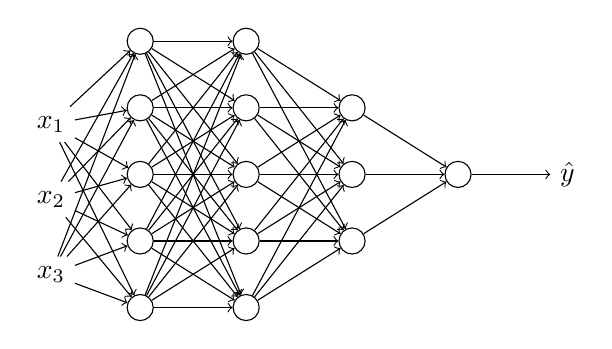
\begin{tikzpicture}[scale=0.25]     \node (x1) at (-2, 1) {$x_1$};
    \node [below = .5 cm of x1] (x2) {$x_2$};
    \node [below = .5 cm of x2] (x3) {$x_3$};
    \node [draw,circle,above right = 1 cm of x1] (n11) {};
    \node [draw,circle,below = .5 cm of n11] (n12) {};
    \node [draw,circle,below = .5cm of n12] (n13) {};
    \node [draw,circle,below = .5cm of n13] (n14) {};
    \node [draw,circle,below = .5cm of n14] (n15) {};
    \node [draw,circle,right = 1 cm of n11] (n21) {};
    \node [draw,circle,below = .5 cm of n21] (n22) {};
    \node [draw,circle,below = .5cm of n22] (n23) {};
    \node [draw,circle,below = .5cm of n23] (n24) {};
    \node [draw,circle,below = .5cm of n24] (n25) {};
    \node [draw,circle,right = 1cm of n22] (n31) {};
    \node [draw,circle,below = .5cm of n31] (n32) {};
    \node [draw,circle,below = .5cm of n32] (n33) {};
    \node [draw,circle,right = 1cm of n32] (outputneuron) {};
    \node [right = 1cm of outputneuron] (yhat) {$\hat y$};
    \draw[->] (x1) to (n11);
    \draw[->] (x1) to (n12);
    \draw[->] (x1) to (n13);
    \draw[->] (x1) to (n14);
    \draw[->] (x1) to (n15);
    \draw[->] (x2) to (n11);
    \draw[->] (x2) to (n12);
    \draw[->] (x2) to (n13);
    \draw[->] (x2) to (n14);
    \draw[->] (x2) to (n15);
    \draw[->] (x3) to (n11);
    \draw[->] (x3) to (n12);
    \draw[->] (x3) to (n13);
    \draw[->] (x3) to (n14);
    \draw[->] (x3) to (n15);
    \draw[->] (n11) to (n21);
    \draw[->] (n11) to (n22);
    \draw[->] (n11) to (n23);
    \draw[->] (n11) to (n24);
    \draw[->] (n11) to (n25);
    \draw[->] (n12) to (n21);
    \draw[->] (n12) to (n22);
    \draw[->] (n12) to (n23);
    \draw[->] (n12) to (n24);
    \draw[->] (n12) to (n25);
    \draw[->] (n13) to (n21);
    \draw[->] (n13) to (n22);
    \draw[->] (n13) to (n23);
    \draw[->] (n13) to (n24);
    \draw[->] (n13) to (n25);
    \draw[->] (n14) to (n21);
    \draw[->] (n14) to (n22);
    \draw[->] (n14) to (n23);
    \draw[->] (n14) to (n24);
    \draw[->] (n14) to (n25);
    \draw[->] (n15) to (n21);
    \draw[->] (n15) to (n22);
    \draw[->] (n15) to (n23);
    \draw[->] (n15) to (n24);
    \draw[->] (n15) to (n25);
    \draw[->] (n21) to (n31);
    \draw[->] (n21) to (n32);
    \draw[->] (n21) to (n33);
    \draw[->] (n22) to (n31);
    \draw[->] (n22) to (n32);
    \draw[->] (n22) to (n33);
    \draw[->] (n23) to (n31);
    \draw[->] (n23) to (n32);
    \draw[->] (n23) to (n33);
    \draw[->] (n24) to (n31);
    \draw[->] (n24) to (n32);
    \draw[->] (n24) to (n33);
    \draw[->] (n25) to (n31);
    \draw[->] (n25) to (n32);
    \draw[->] (n25) to (n33);
    \draw[->] (n31) to (outputneuron);
    \draw[->] (n32) to (outputneuron);
    \draw[->] (n33) to (outputneuron);
    \draw[->] (outputneuron) to (yhat);
  \end{tikzpicture}
  \caption{Four-layer, fully connected neural network.} \end{figure}
In our example depicted, $n^{[0]} = n_x = 3$, $n^{[1]} = n^{[2]} = 5$ and $n^{[3]} = 3$ and $n^{L} = 1$. We'll also use $a^{[\ell]} = g^{[\ell]}(z^{[\ell]})$ to denote the activations in layer $\ell$, where to compute $z^{[\ell]}$ we use weights matrix $W^{[\ell]}$ and bias term $b^{[\ell]}$. Lastly, realize that with this notation our input matrix $X = a^{[0]}$ and our output $\hat y = a^{[L]}$.

\paragraph{Forward Propagation}
In general, we have that for a single training example:
\begin{align*}   z^{[\ell]} &= W^{[\ell]} a^{[\ell-1]} + b^{[\ell]}, \\ 
  a^{[\ell]} &= g^{[\ell]}(z^{[\ell]}). \end{align*}
And for our entire training set, where $X = A^{[0]}$ is our data arranged such that each column is an observation:
\begin{align}   Z^{[\ell]} &= W^{[\ell]} A^{[\ell-1]} + b^{[\ell]}, \\ 
  A^{[\ell]} &= g^{[\ell]}(Z^{[\ell]}).    \end{align}
Note that by rules of matrix multiplication, it's easy to see that $Z^{[\ell]}$ must have as many columns as there are training examples, and since $g^{[\ell]}$ is applied element-wise then $A^{[\ell]}$ also has as $m$ columns.
For our last layer, $\hat Y = g(Z^{[L]}) = A^{[L]}$. We remark that although we typically try to vectorize code and remove \texttt{for}-loops, it is perfectly reasonable to loop over the layers in the network during forward propagation. I.e. we expect to see \texttt{for} $\ell = 1, \ldots, L$.

\paragraph{Getting Your Dimensions Right} In general, the dimension for a weights matrix at layer $\ell$ is given b
\begin{equation}   W^{[\ell]} : \left( n^{[\ell]}, n^{[\ell - 1]} \right). \end{equation}
What about our bias term? In general, $b^{[\ell]} : \left(n^{[\ell]}, 1\right)$, Further, during backpropogation, the dimensions of the derivative matrices don't change. I.e. 
$\d   W^{[\ell]} : \left( n^{[\ell]}, n^{[\ell - 1]} \right)$, and $\d b^{[\ell]} : \left(n^{[\ell]}, 1\right)$.

\paragraph{Deep Representations}
What do our intermediary layers come to learn in different applications?

Consider face detection. The first layer of the network may learn to detect edges, and the second layer perhaps may learn how to detect different pieces of a face by connecting edges together such as an eye or an ear. A later layer of a network may learn to distinguish between faces at an even less granular level.

As another example consider problems in the context of audio. The first layer of the network may lrn to distinguish between low and high frequency waveforms, whereas the second layer may learn to recognize phonemes (in the word cat, each letter, when pronounced, is a phoneme), and later layers of the network may learn to recognize words and finally phrases/sentences.

Earlier layers are in general based on more granular features, i.e. simple transformations of the input data. Later layers compose hierarchically and are eventually able to solve complex tasks.

\paragraph{Circuit Theory and Deep Learning}
``There are functions you can compute with a 'small' $L$-layer deep neural network that shallower networks require exponentially more hidden units to compute.''

As an example, consider using a neural network to approximate \texttt{xor} applied to $n$ input bits. I.e. we seek to calculate $x_1 \textrm{ xor } x_2 \textrm{ xor } \ldots \textrm{ xor } x_n$. If we are free to use as many layers in the network as we wish, then we could envision building a \texttt{xor} tree as follows: pair successive inputs together and apply the \texttt{xor} operation, and pipe the resulting output into the subsequent layer of the network. Realize that we require $\log n$ layers in our network in order to exactly compute the right answer. If, on the other hand, we weren't allowed to use an arbitrary number of layers but instead only a single hidden layer, we would require $O(2^n)$ neurons in order to achieve the same result; to see why realize that we effectively need to enumerate all possible $2^n$ possible input sequences in order to map them correctly back to the right answer in a subsequent step. Note that it is possible to get away with using only $2^{n-1}$ neurons to accomplish this task but this is still exponentially more neurons than the network with $O(\log n)$ layers.

\paragraph{Building Blocks of Deep Neural Networks} A.

\end{document}

